\subsection{Funcionamiento general}

 %% Texto del cuerpo del documento
 En la ilustración \ref{fg:diagflujo}, se muestra un diagrama de flujo, el cual busca simplificar el funcionamiento general del sistema de compostaje, enlazando cada uno de los módulos y cómo será su orden dentro del proceso de compostaje. 

%% Insertar una imagen 
        \begin{figure}[h!]
            \centering
            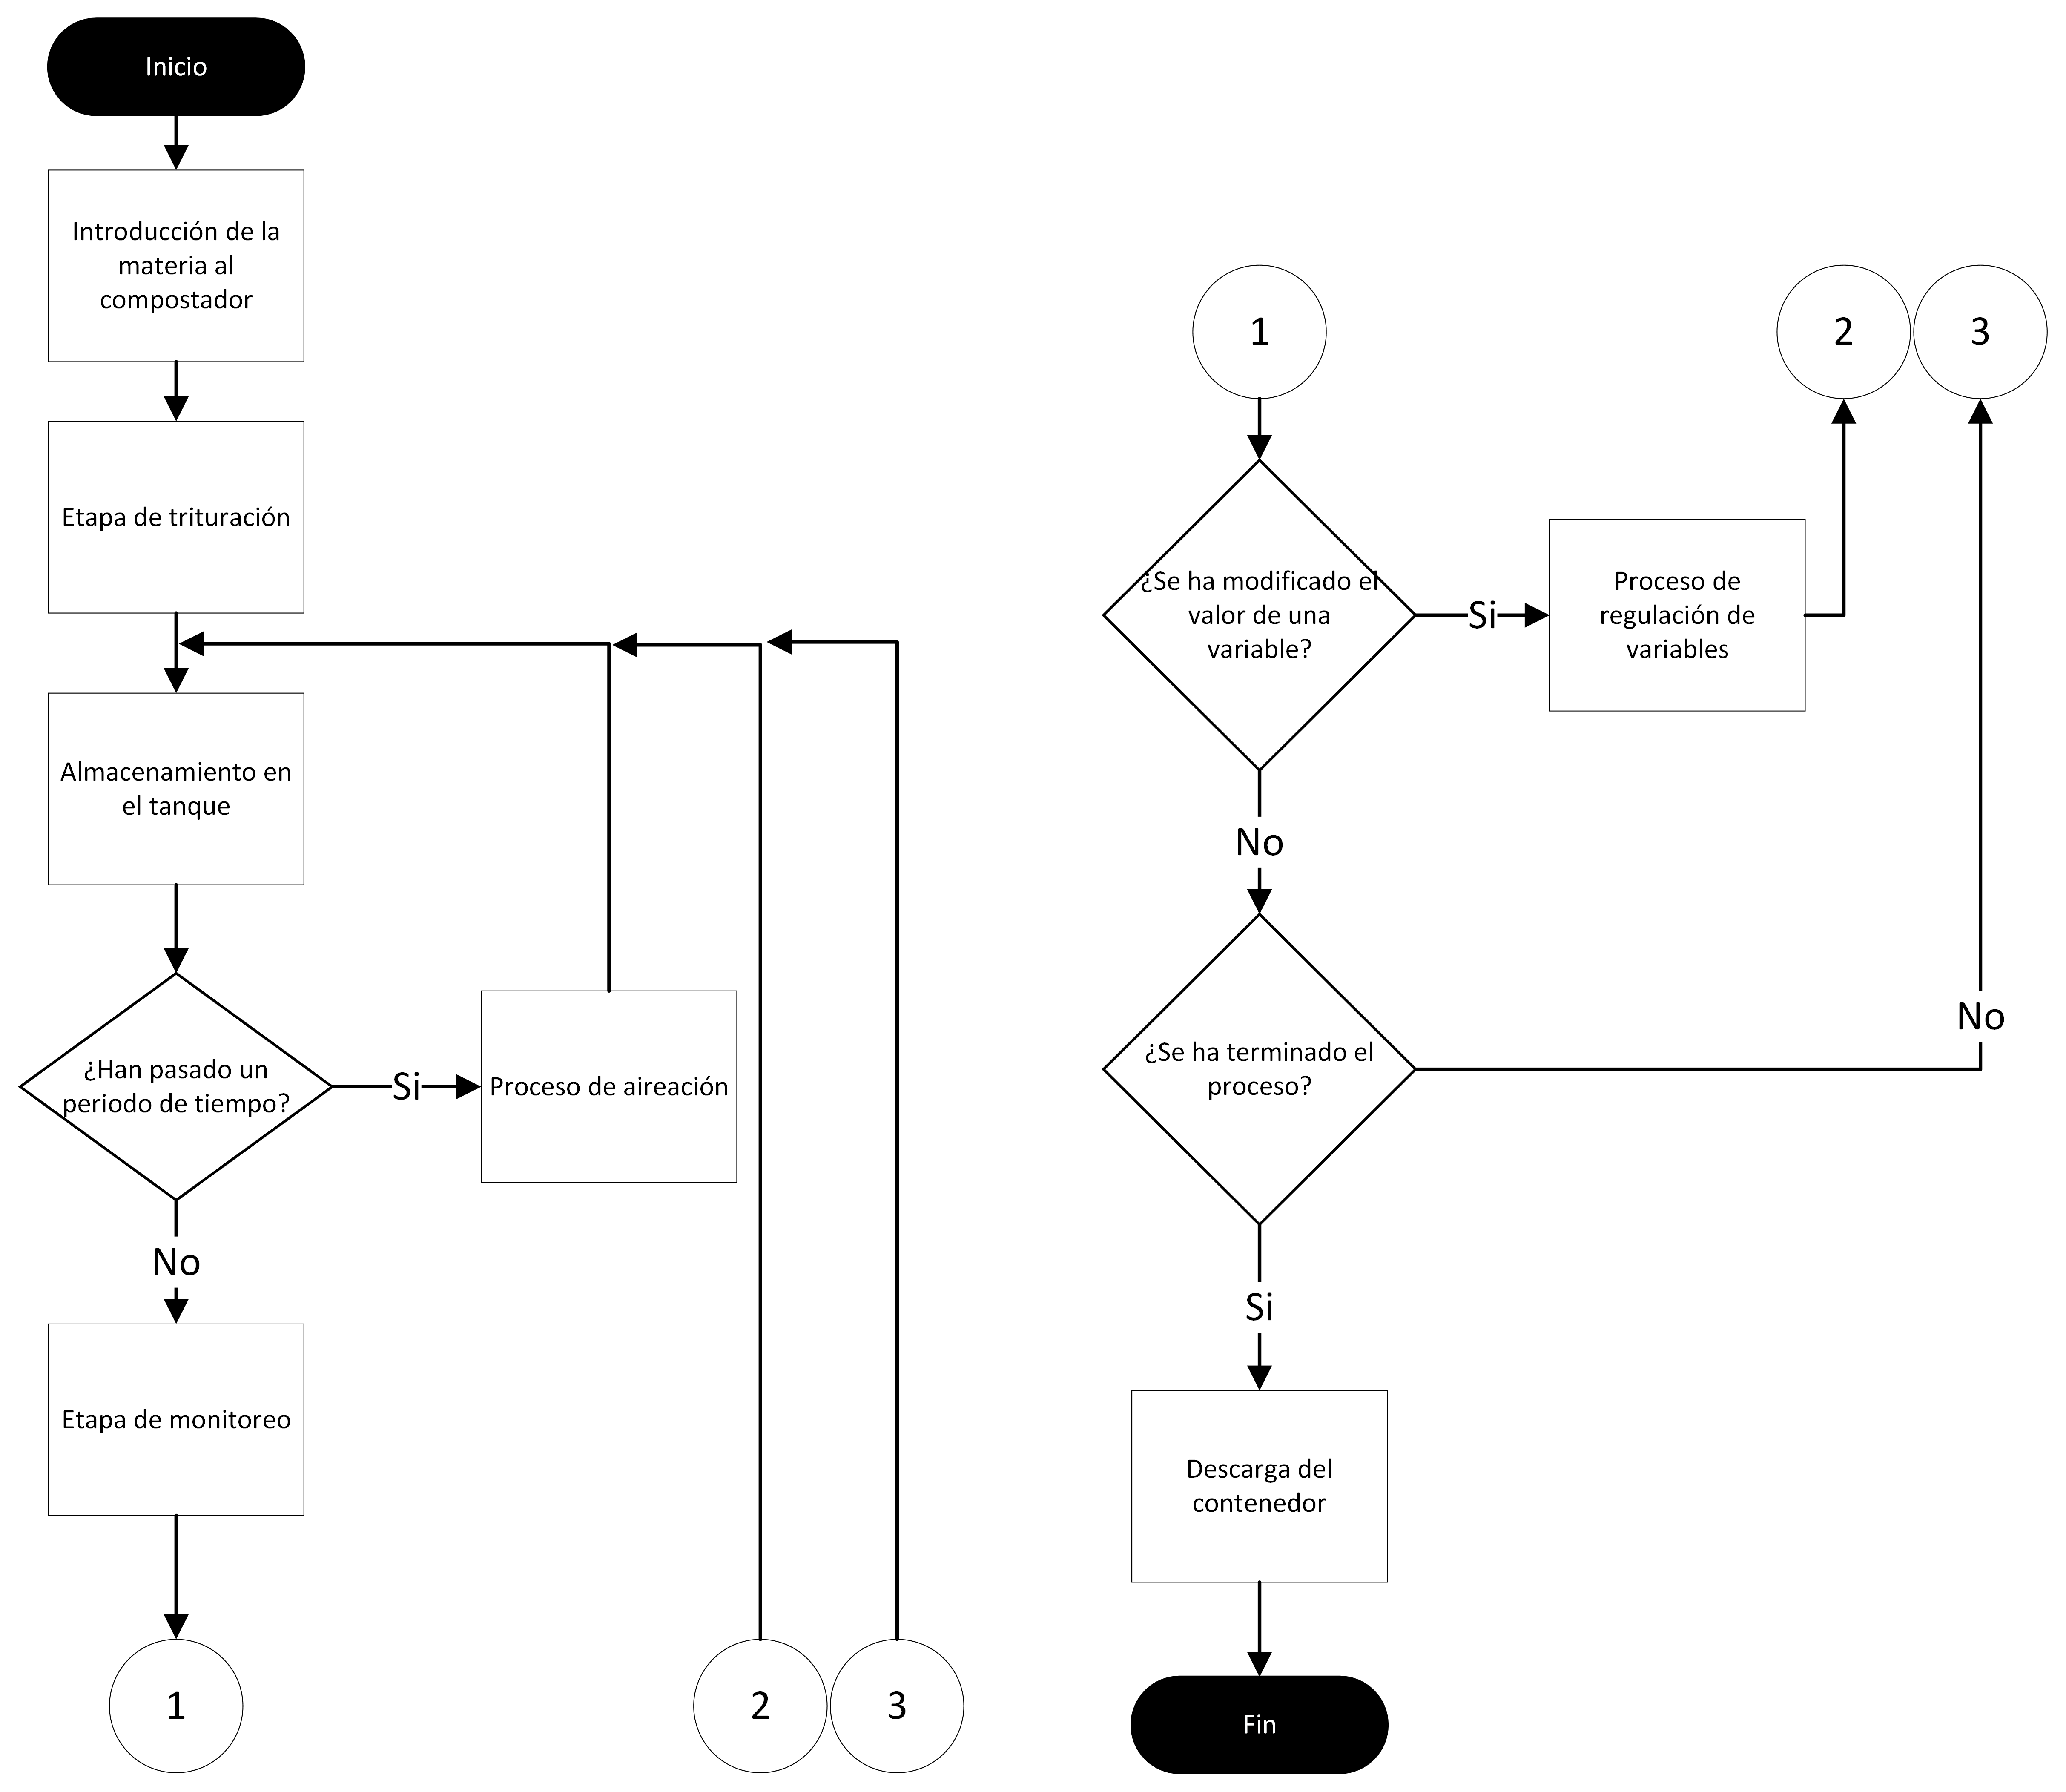
\includegraphics[scale=0.25]{images/Capitulo 3/Presentacion del proceso/Diagrama de flujo del sistema.png}
            \caption{Diagrama de flujo del funcionamiento general del sistema}
            \label{fg:diagflujo}
        \end{figure}
        
 El primer módulo que se presenta corresponde a la “Introducción de la materia al compostador”. Esta carga de materia se hace de forma manual, vertiendo la materia orgánica por un conducto especial que va enlazado a la etapa de trituración.
 
Se plantea que la etapa de trituración sea ejecutada de forma manual, de manera que sea el esfuerzo del usuario el que realice el movimiento del sistema de trituración con ayuda de un sistema mecánico de transmisión de movimiento.

La etapa de almacenamiento hace referencia al espacio donde se va a realizar el proceso de compostaje, ya que el método In-Vessel requiere de un contenedor dentro del cual se pueda adaptar el ambiente necesario para el crecimiento de microorganismos.

Dentro del recipiente de almacenaje, se realizará la etapa de control, a partir de una subetapa de monitoreo y una regulación. Con ayuda de diversos sensores, se busca monitorear el estado de las variables y, si es necesario, con ayuda de diversos actuadores, se busca regularlas dentro de unos parámetros determinados de forma automática.

Otro proceso en paralelo es la etapa de agitación. Esta etapa se encarga de mover la materia orgánica; es un proceso necesario para oxigenar a los microorganismos y lograr la homogeneización del compost. Este proceso se realiza cada cierto periodo de tiempo de forma automática.

Por último, la etapa de descarga del compost se hará a través de una de las laterales del contenedor. Esta etapa se realiza de manera manual.